\documentclass{beamer}

\usefonttheme{professionalfonts} % using non standard fonts for beamer
\usefonttheme{serif} % default family is serif

\usepackage{hyperref}
%\usepackage{minted}
\usepackage{animate}
\usepackage{graphicx}
\def\Put(#1,#2)#3{\leavevmode\makebox(0,0){\put(#1,#2){#3}}}
\usepackage{colortbl}
\usepackage{tikz}
\usepackage{amssymb}
\usepackage{enumerate}
\usepackage{arydshln}
\usepackage{algorithm}
\usepackage{algpseudocode}

\colorlet{lightred}{red!25}
\colorlet{lightgreen}{green!25}


\newcommand\blfootnote[1]{%

  \begingroup

  \renewcommand\thefootnote{}\footnote{#1}%

  \addtocounter{footnote}{-1}%

  \endgroup

}

\makeatletter

%%%%%%%%%%%%%%%%%%%%%%%%%%%%%% Textclass specific LaTeX commands.

 % this default might be overridden by plain title style

 \newcommand\makebeamertitle{\frame{\maketitle}}%

 % (ERT) argument for the TOC

 \AtBeginDocument{%

   \let\origtableofcontents=\tableofcontents

   \def\tableofcontents{\@ifnextchar[{\origtableofcontents}{\gobbletableofcontents}}

   \def\gobbletableofcontents#1{\origtableofcontents}

 }

%%%%%%%%%%%%%%%%%%%%%%%%%%%%%% User specified LaTeX commands.

\usetheme{Malmoe}

% or ...

\useoutertheme{infolines}

\addtobeamertemplate{headline}{}{\vskip2pt}

\setbeamercovered{transparent}

% or whatever (possibly just delete it)

\makeatother

\begin{document}
\title[PFLOCK report]{PFLOCK Report}
\author[AC]{Andres Calderon}
\institute[Fall'19]{University of California, Riverside}
\makebeamertitle
\newif\iflattersubsect

\AtBeginSection[] {
    \begin{frame}<beamer>
    \frametitle{Outline} 
    \tableofcontents[currentsection]  
    \end{frame}
    \lattersubsectfalse
}

\AtBeginSubsection[] {
    \begin{frame}<beamer>
    \frametitle{Outline} 
    \tableofcontents[currentsubsection]  
    \end{frame}
}

\begin{frame}{A critical issue in the new approach...}
    \begin{itemize}
        \item Using an example with $\varepsilon=50$, $\mu=5$ and $\delta=5$
        \item Tracking trajectory $13805563$ to illustrate the problem...
    \end{itemize}

\end{frame}

\begin{frame}{Disks at $t_0$}
    \centering
    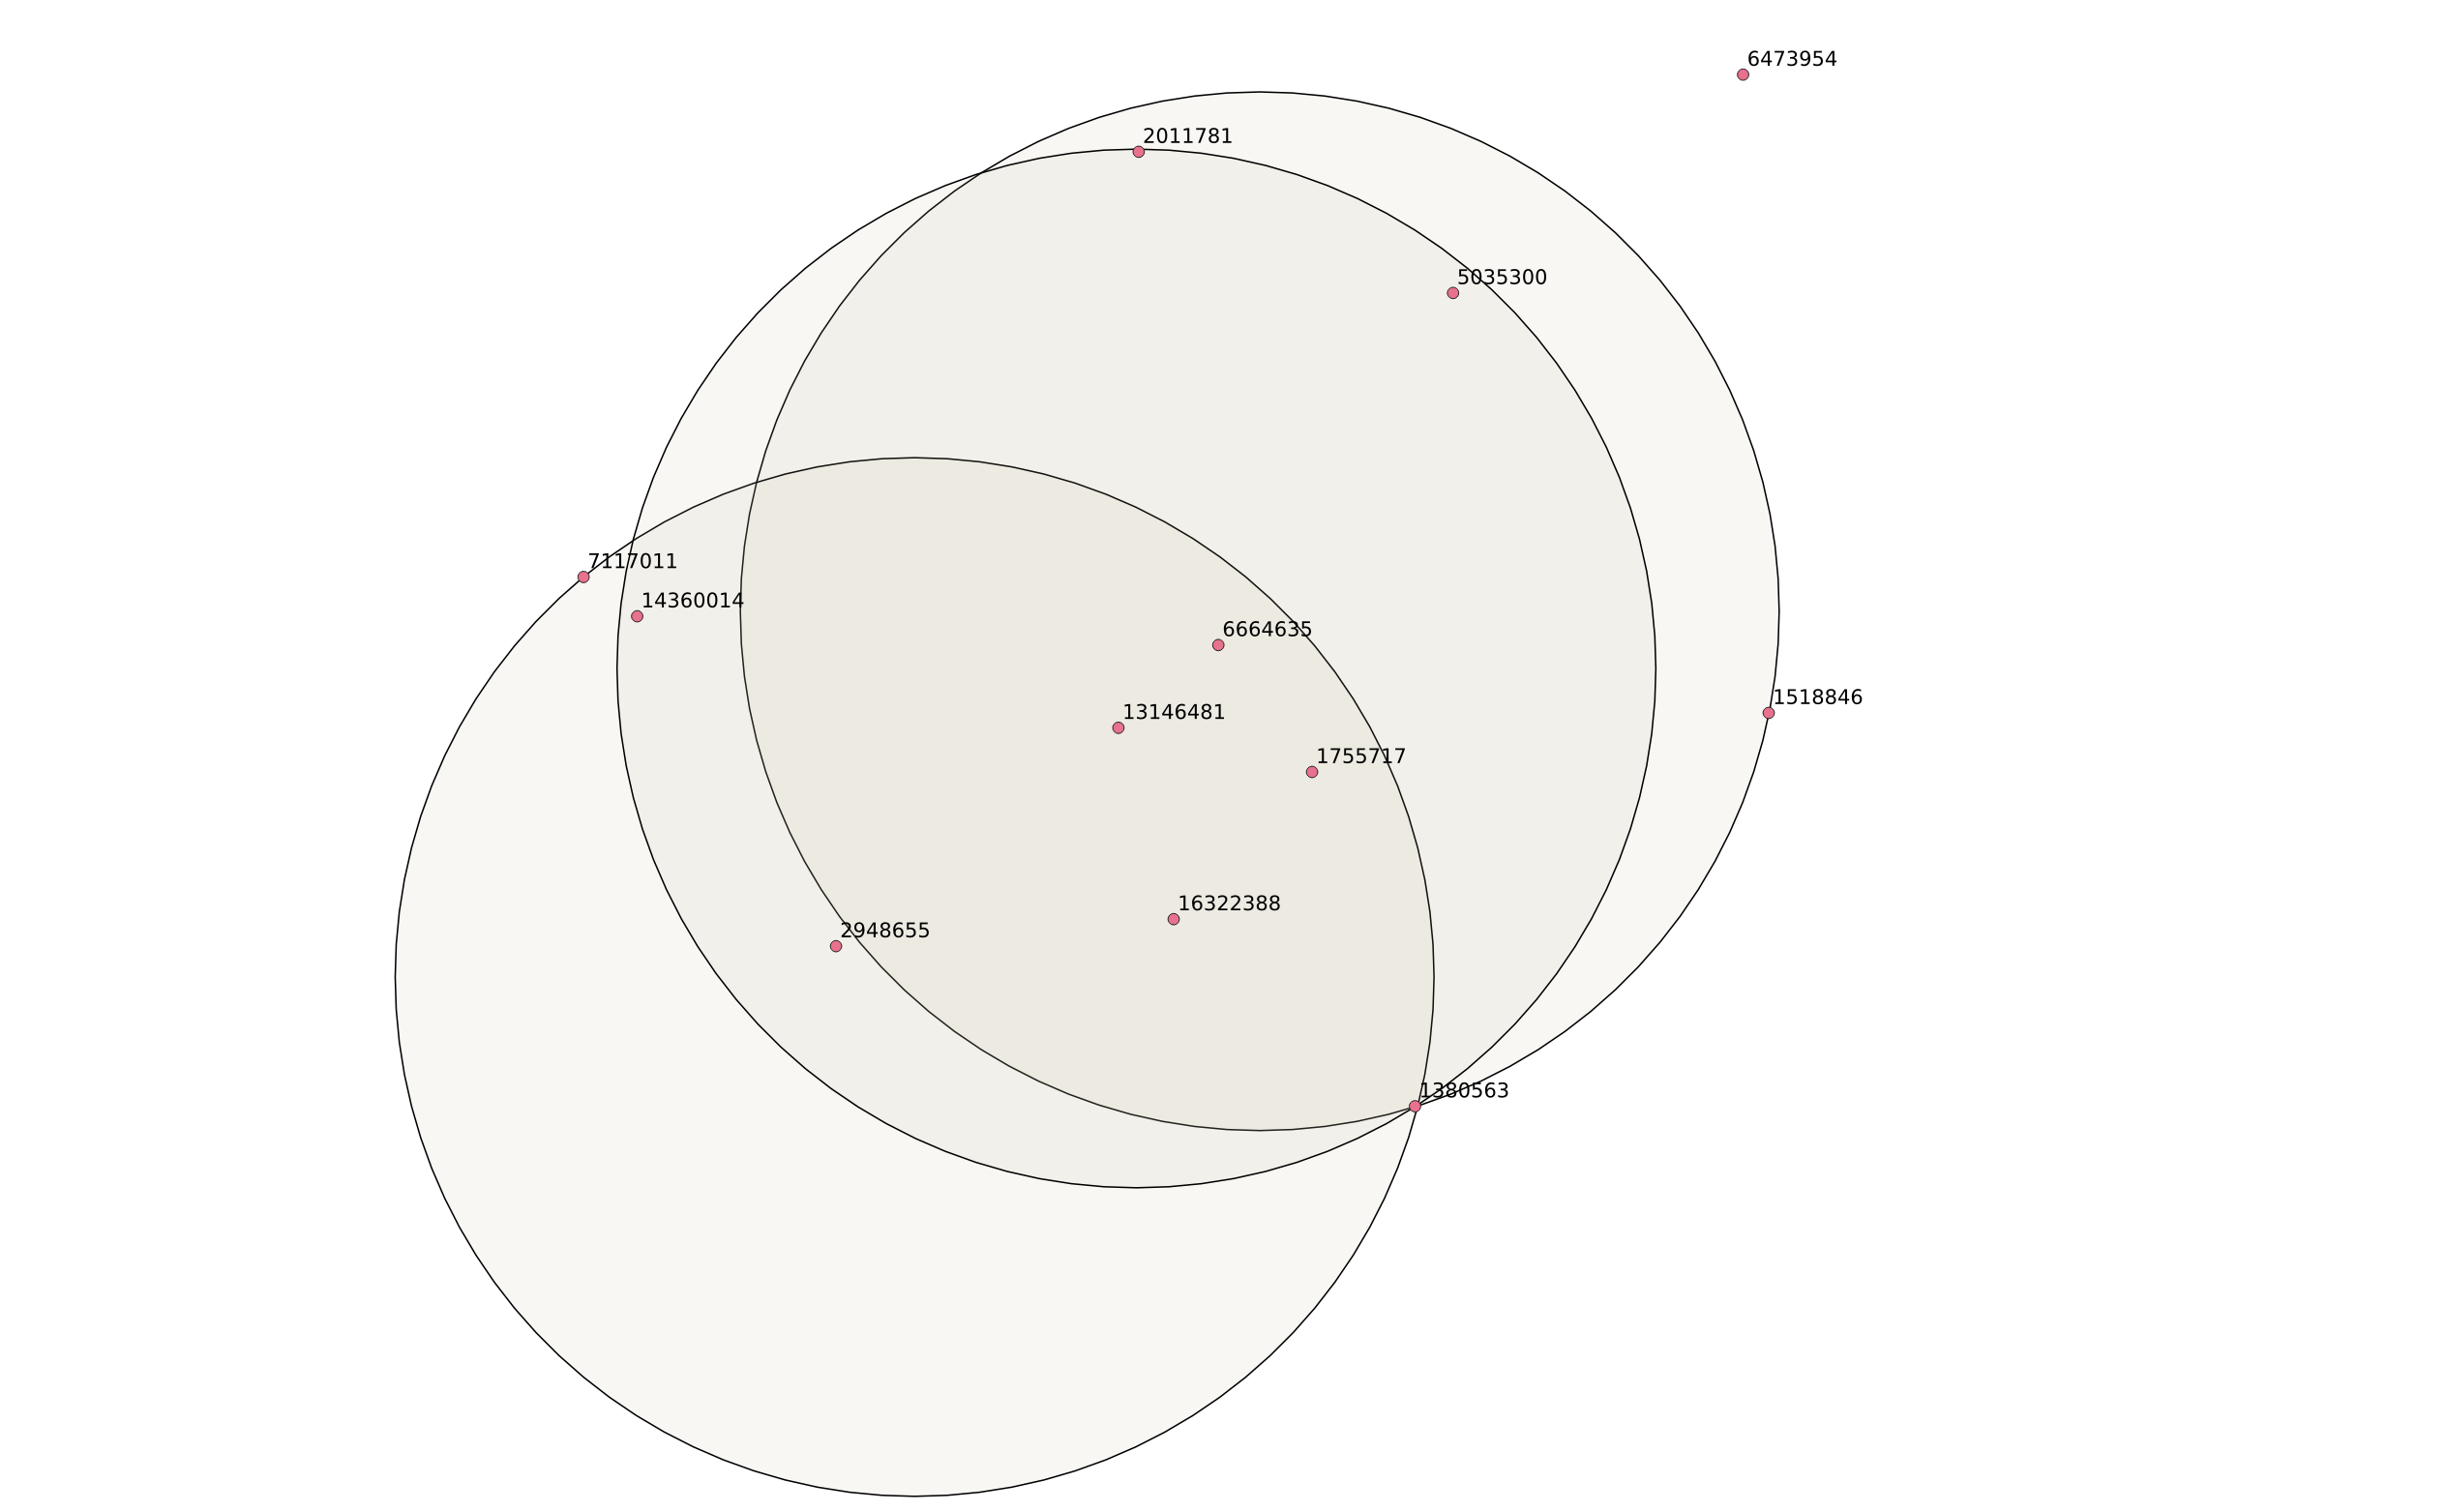
\includegraphics[trim={6cm 0cm 6cm 1.5cm},clip,width=0.65\linewidth]{Figures/t0}
    \scalebox{0.5}{
    \begin{tabular}{c l} \hline
        t& Trajectories in the same disk that \textbf{13805563} \\ \hline
        0&	1518846 1755717 2011781 2948655 5035300 6664635 13146481 16322388 \\
        0&	1755717 2948655 6664635 7117011 13146481 14360014 16322388 \\
        0&	1755717 2011781 2948655 5035300 6664635 13146481 14360014 16322388 \\
        \hline
    \end{tabular}
    }
\end{frame}
\begin{frame}{Disks at $t_1$}
    \centering
    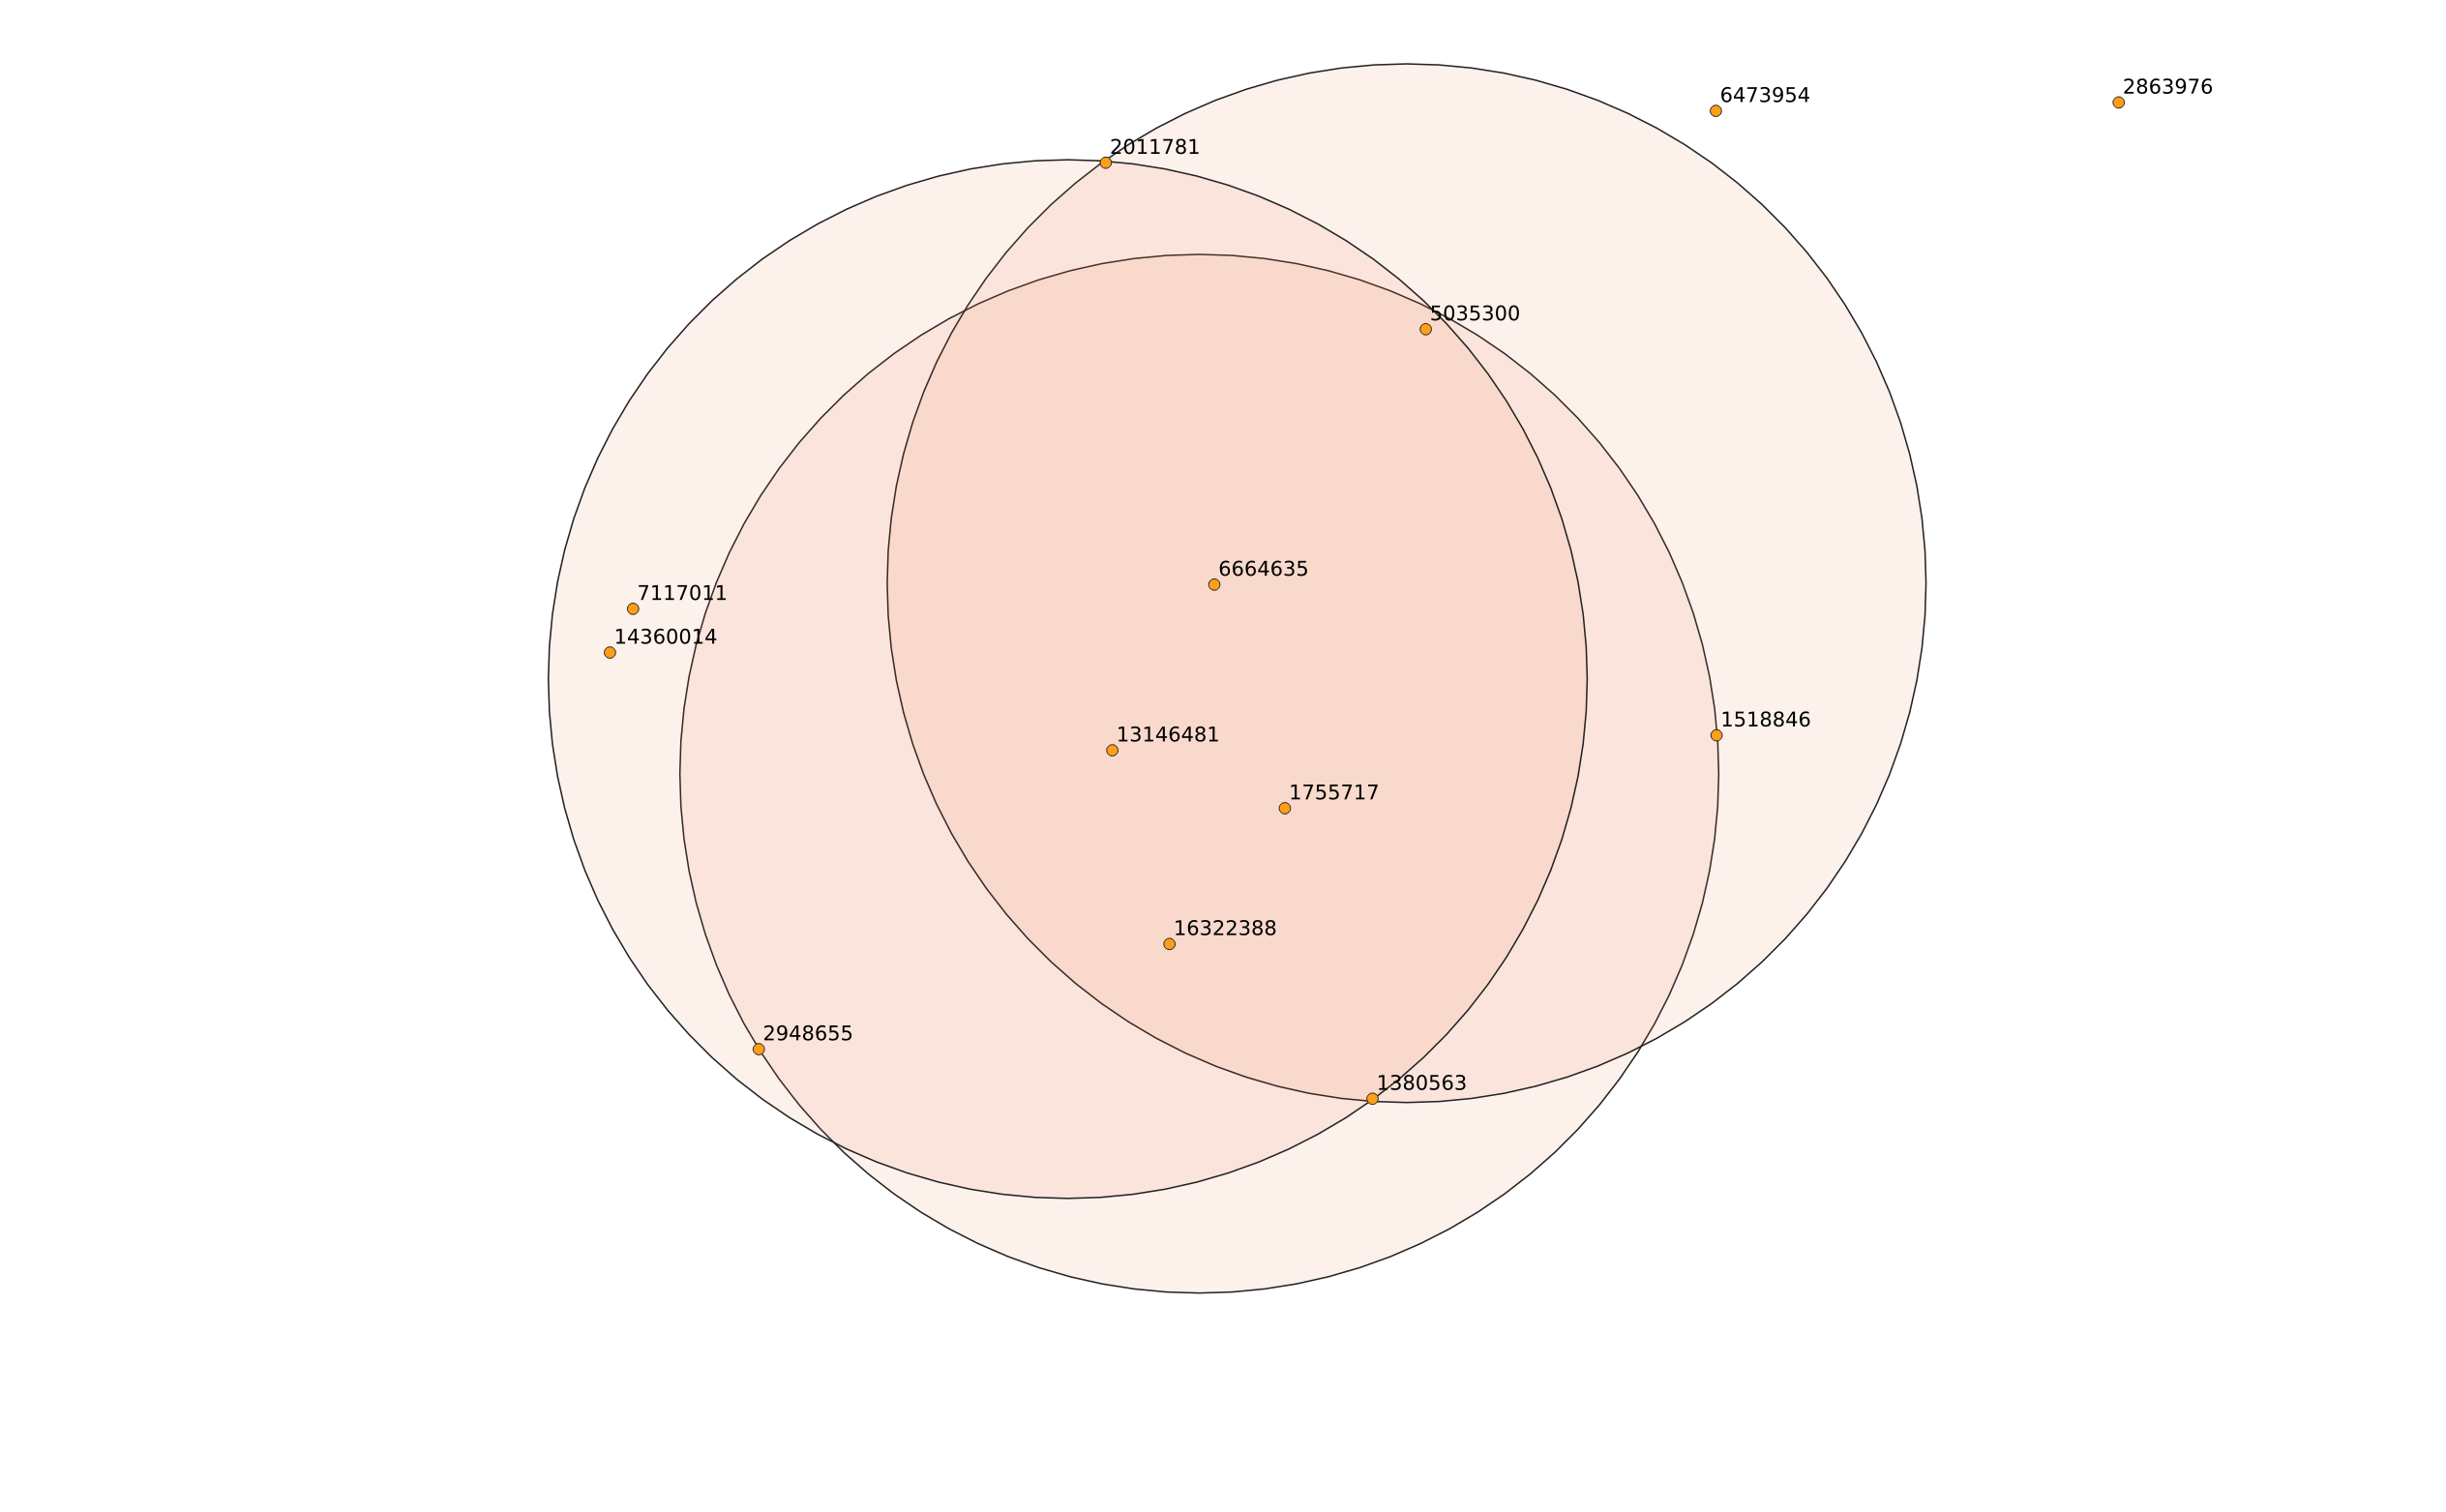
\includegraphics[trim={6cm 1.5cm 6cm 0cm},clip,width=0.65\linewidth]{Figures/t1}
    \scalebox{0.5}{
    \begin{tabular}{c l} \hline
        t& Trajectories in the same disk that \textbf{13805563} \\ \hline
        1&	1518846 1755717 2948655 5035300 6664635 13146481 16322388 \\
        1&	1518846 1755717 2011781 5035300 6664635 13146481 16322388 \\
        1&	1755717 2011781 2948655 5035300 6664635 7117011 13146481 14360014 16322388 \\
        \hline
    \end{tabular}
    }
\end{frame}
\begin{frame}{Disks at $t_2$}
    \centering
    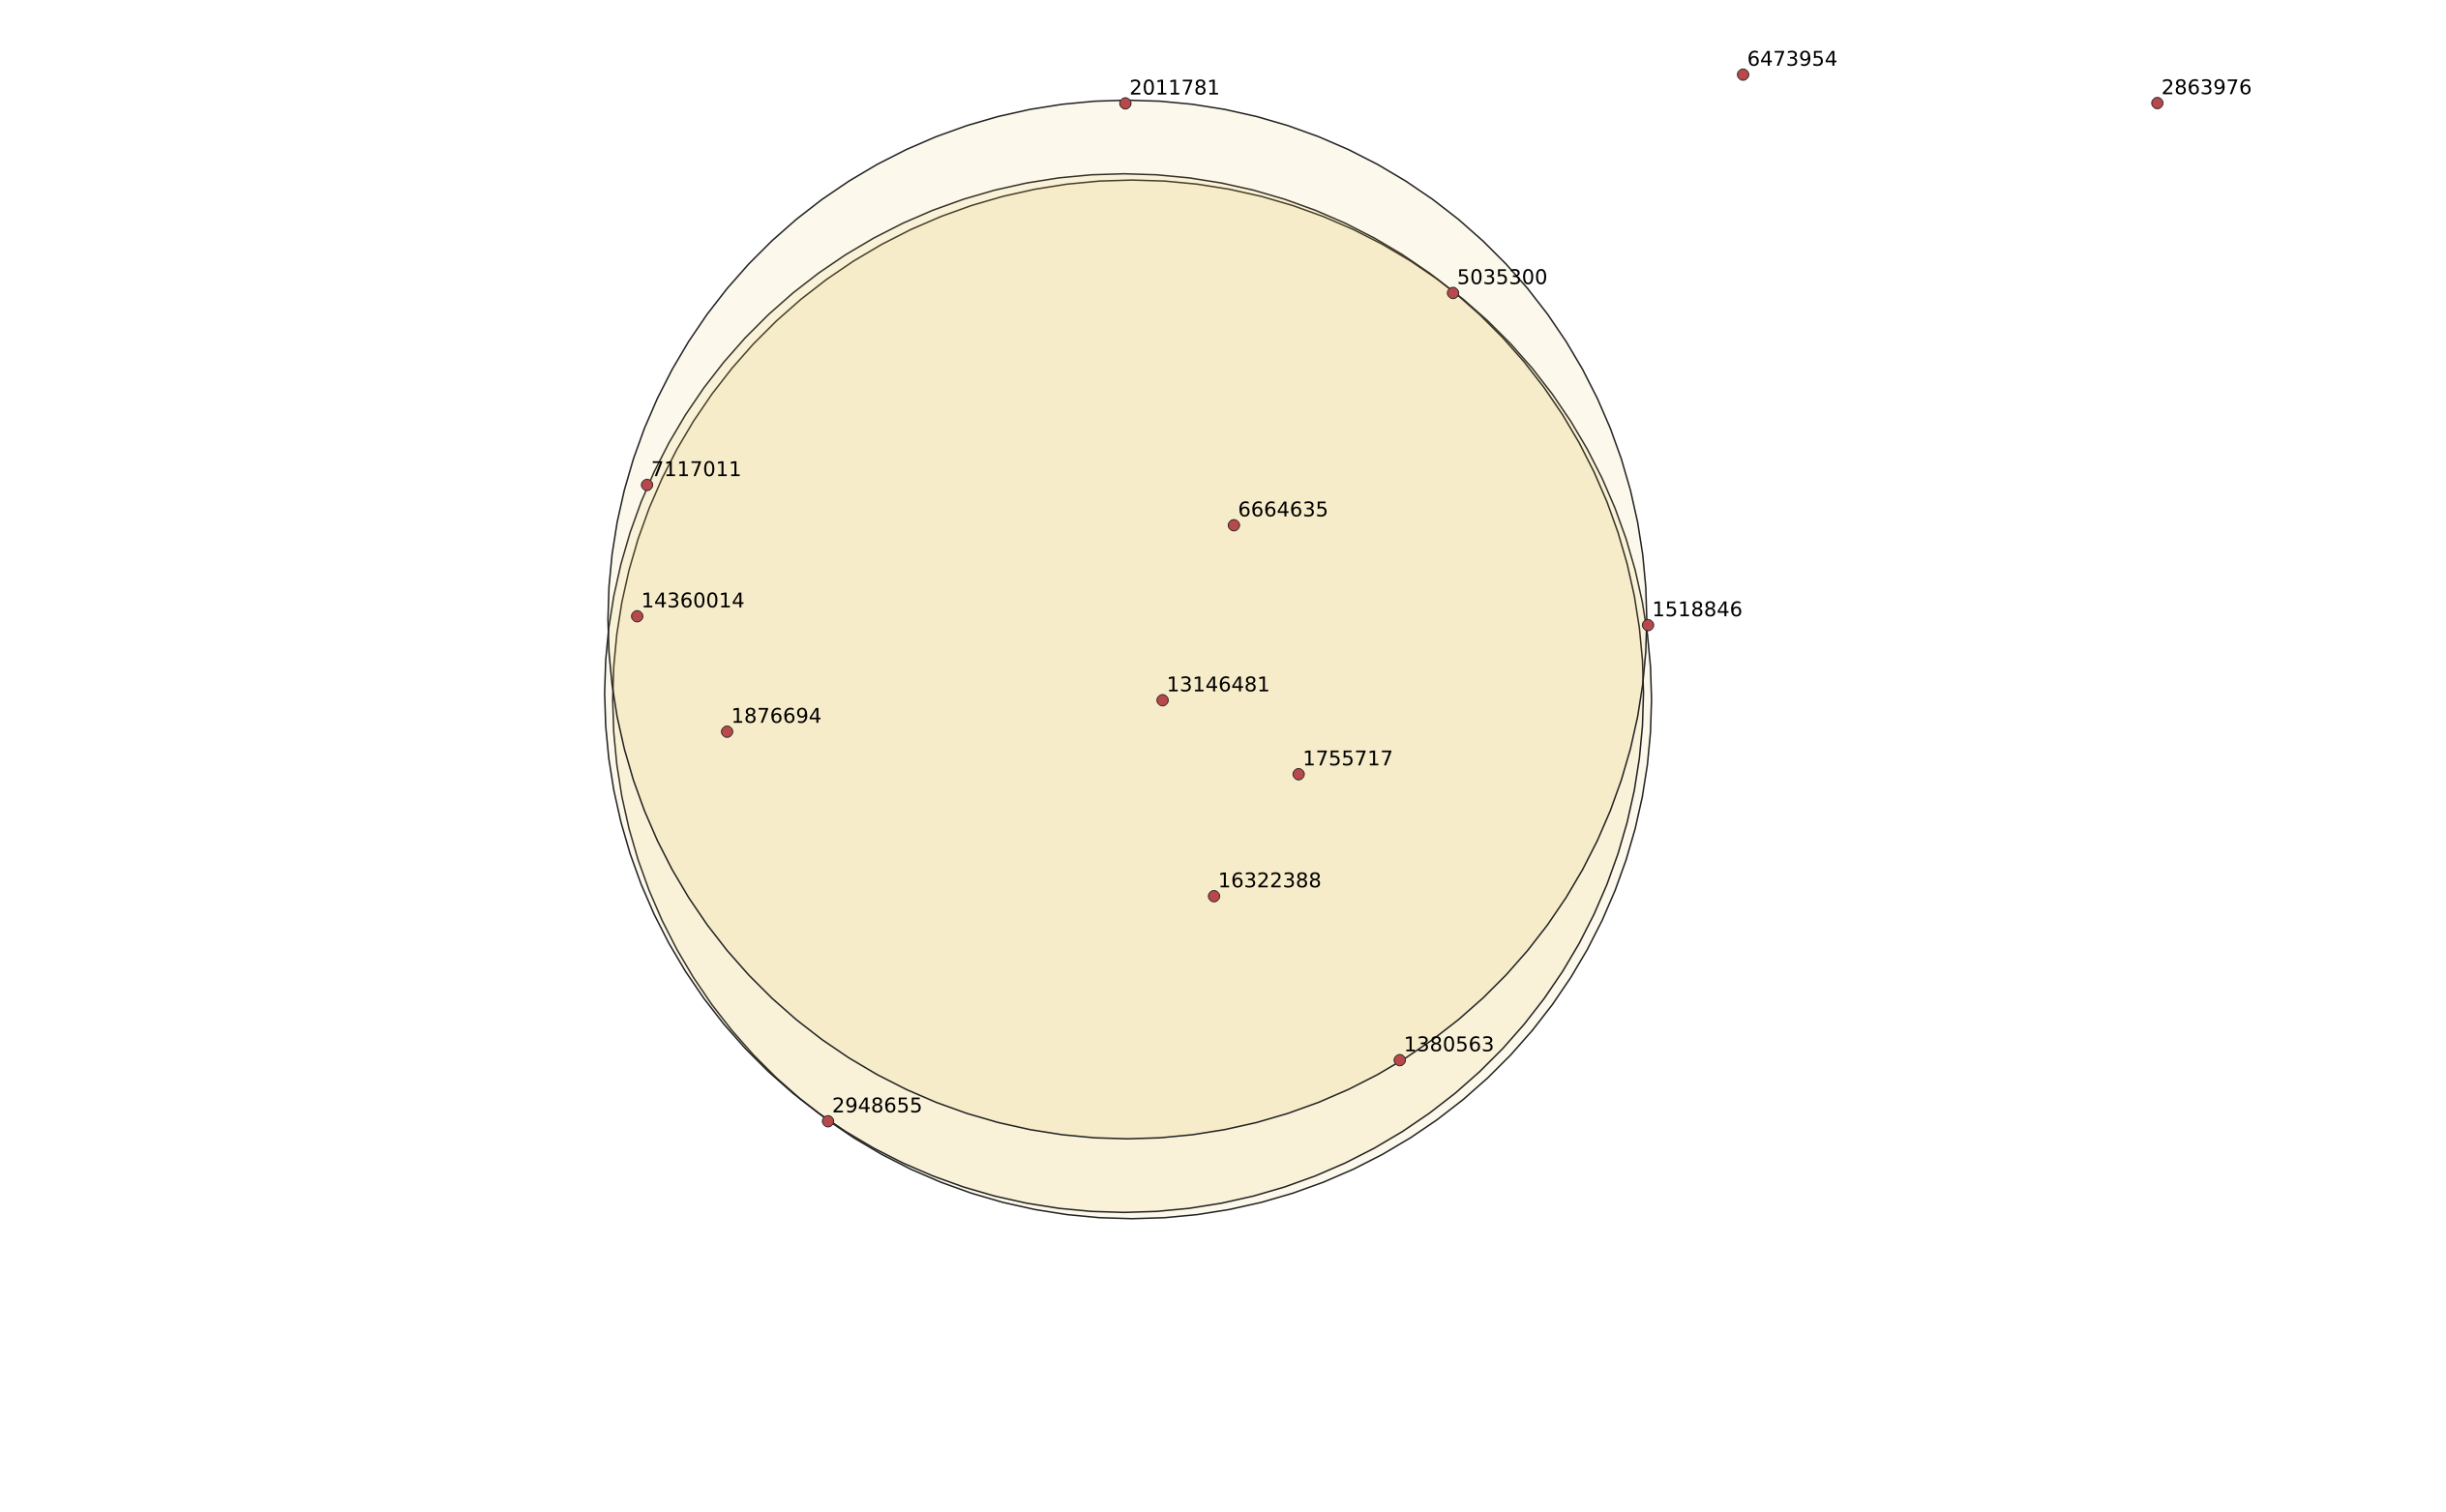
\includegraphics[trim={6cm 2.25cm 6cm 0cm},clip,width=0.7\linewidth]{Figures/t2}
    \scalebox{0.5}{
    \begin{tabular}{c l} \hline
        t& Trajectories in the same disk that \textbf{13805563} \\ \hline
        2&	1518846 1755717 1876694 2011781 5035300 6664635 7117011 13146481 14360014 16322388 \\
        2&	1518846 1755717 1876694 2948655 5035300 6664635 13146481 14360014 16322388 \\
        2&	1755717 1876694 2948655 5035300 6664635 7117011 13146481 14360014 16322388 \\
        \hline
    \end{tabular}
    }
\end{frame}
\begin{frame}{Disks at $t_3$}
    \centering
    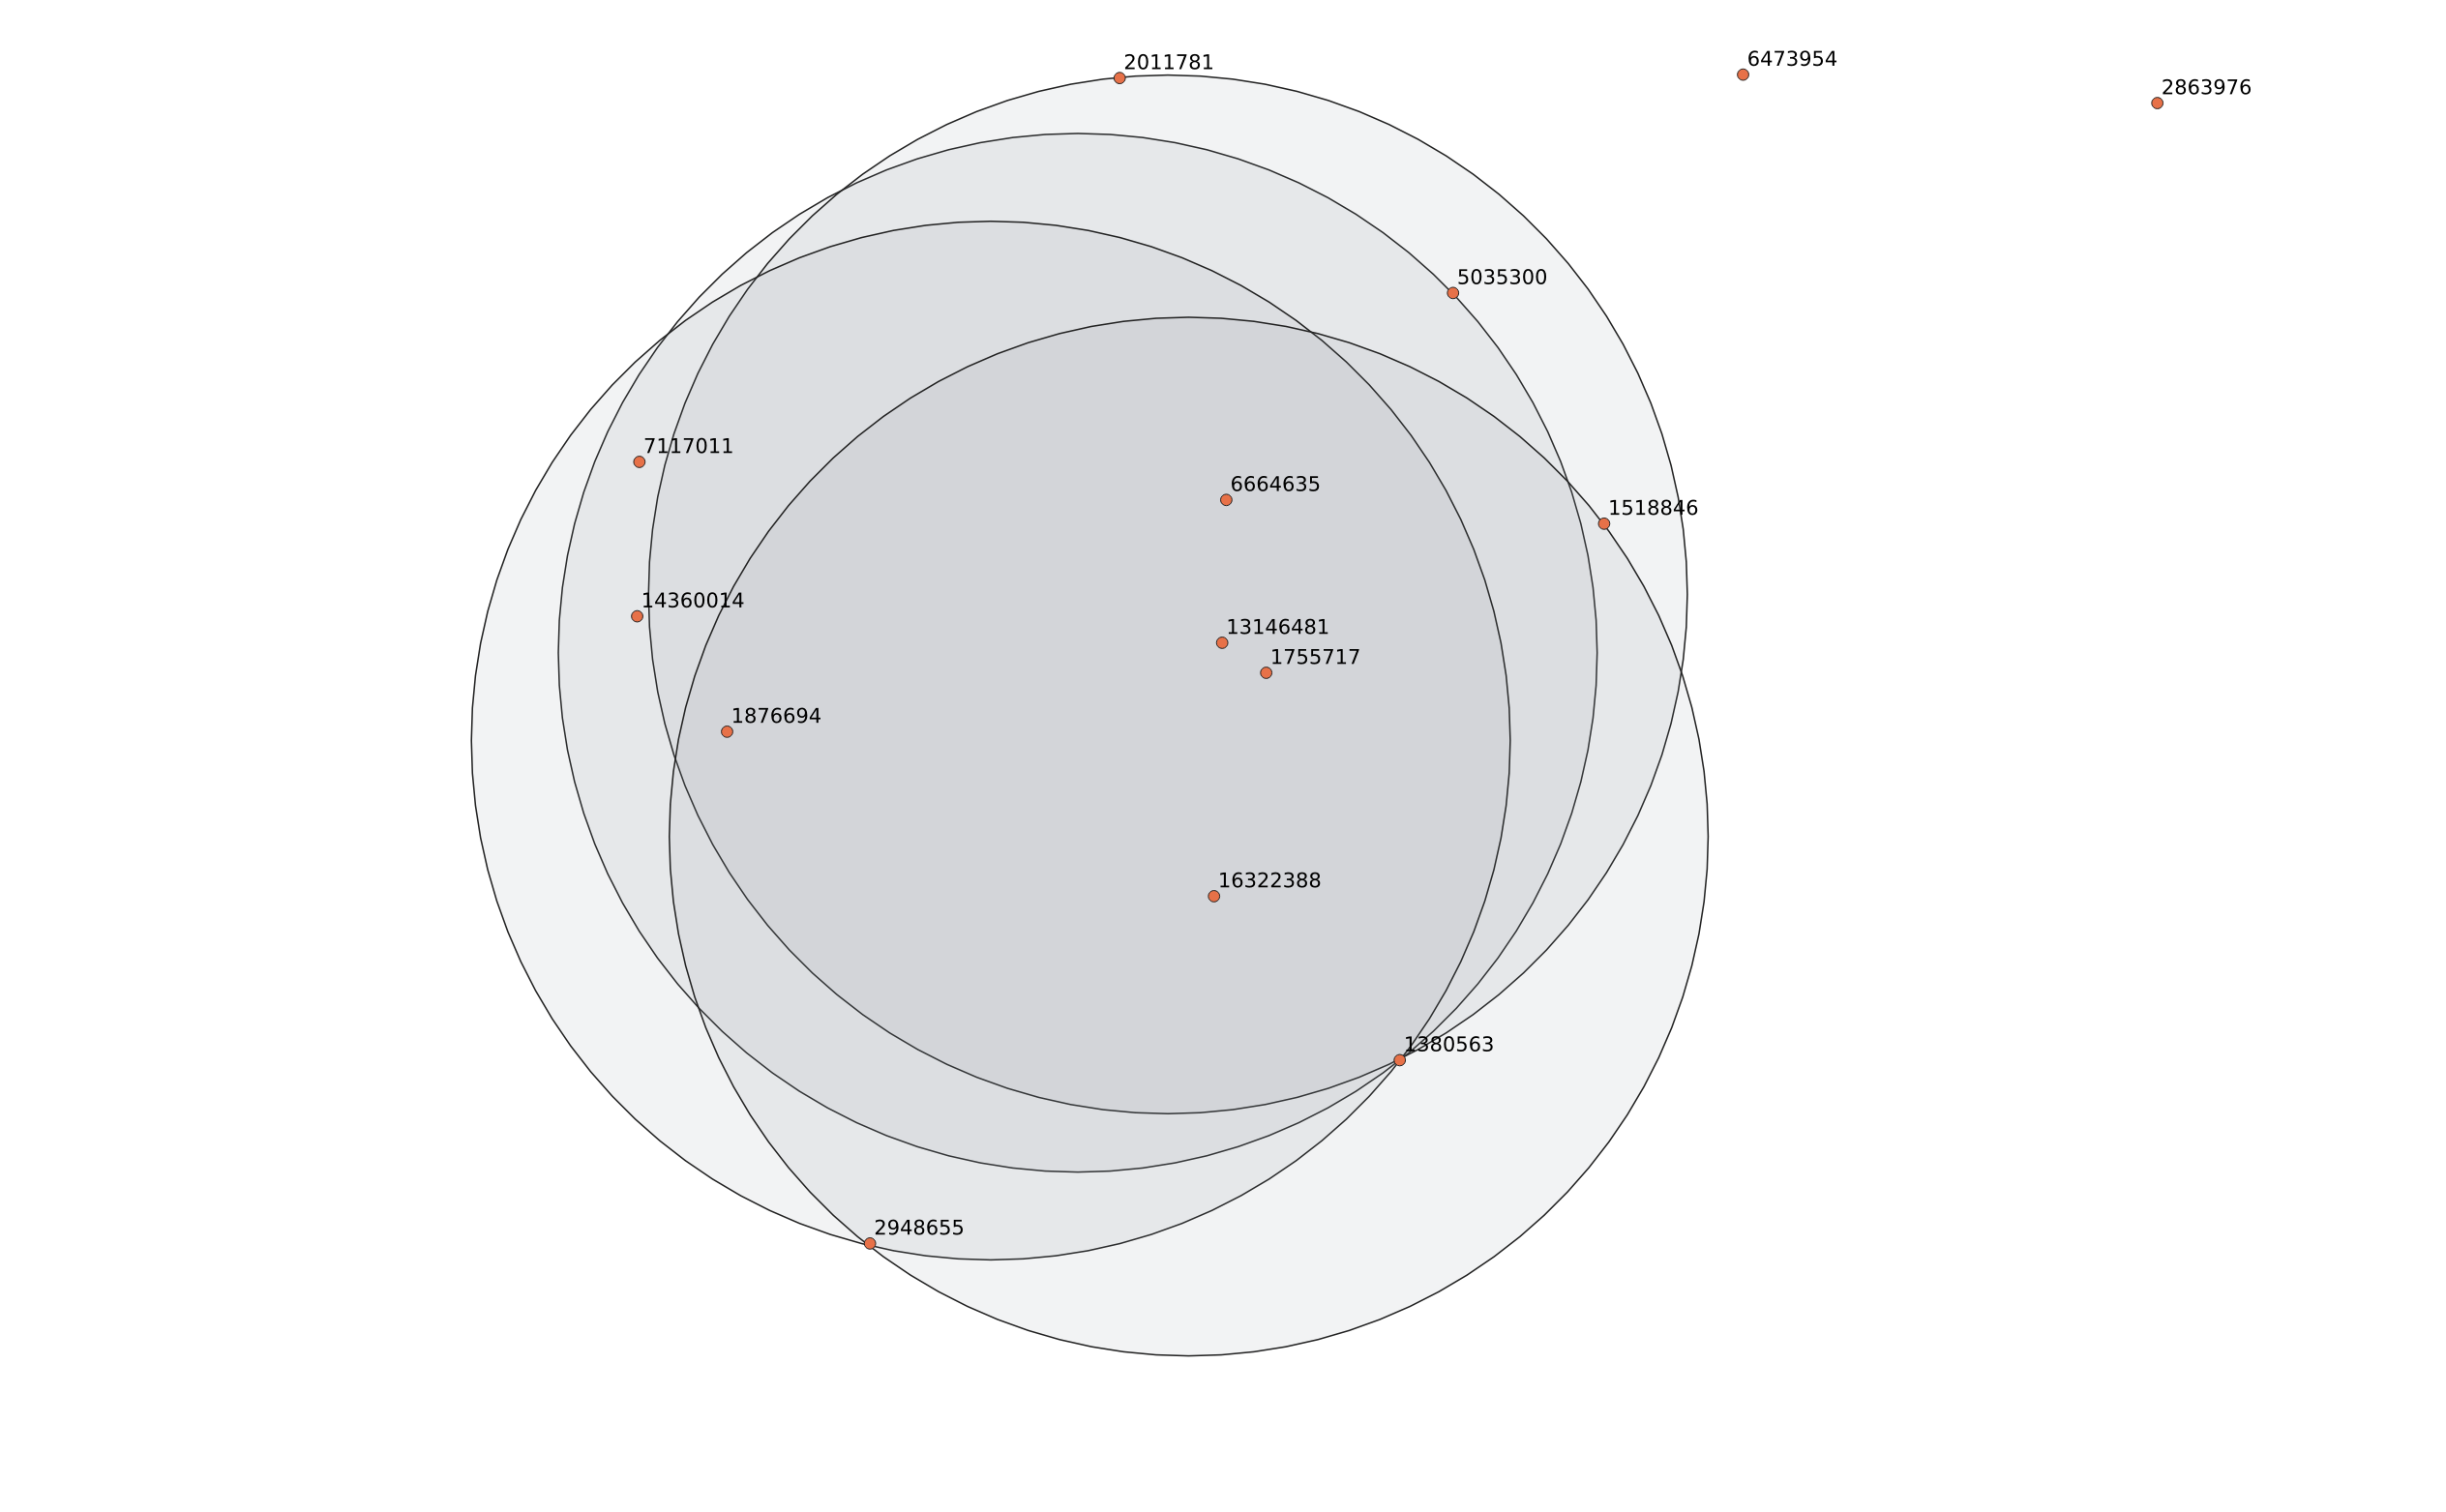
\includegraphics[trim={6cm 2.25cm 6cm 0cm},clip,width=0.7\linewidth]{Figures/t3}
    \scalebox{0.5}{
    \begin{tabular}{c l} \hline
        t& Trajectories in the same disk that \textbf{13805563} \\ \hline
        3&	1518846 1755717 1876694 5035300 6664635 7117011 13146481 14360014 16322388 \\
        3&	1518846 1755717 1876694 2011781 5035300 6664635 13146481 16322388 \\
        3&	1518846 1755717 1876694 2948655 6664635 13146481 16322388 \\
        3&	1755717 1876694 2948655 6664635 7117011 13146481 14360014 16322388 \\
        \hline
    \end{tabular}
    }
\end{frame}
\begin{frame}{Disks at $t_4$}
    \centering
    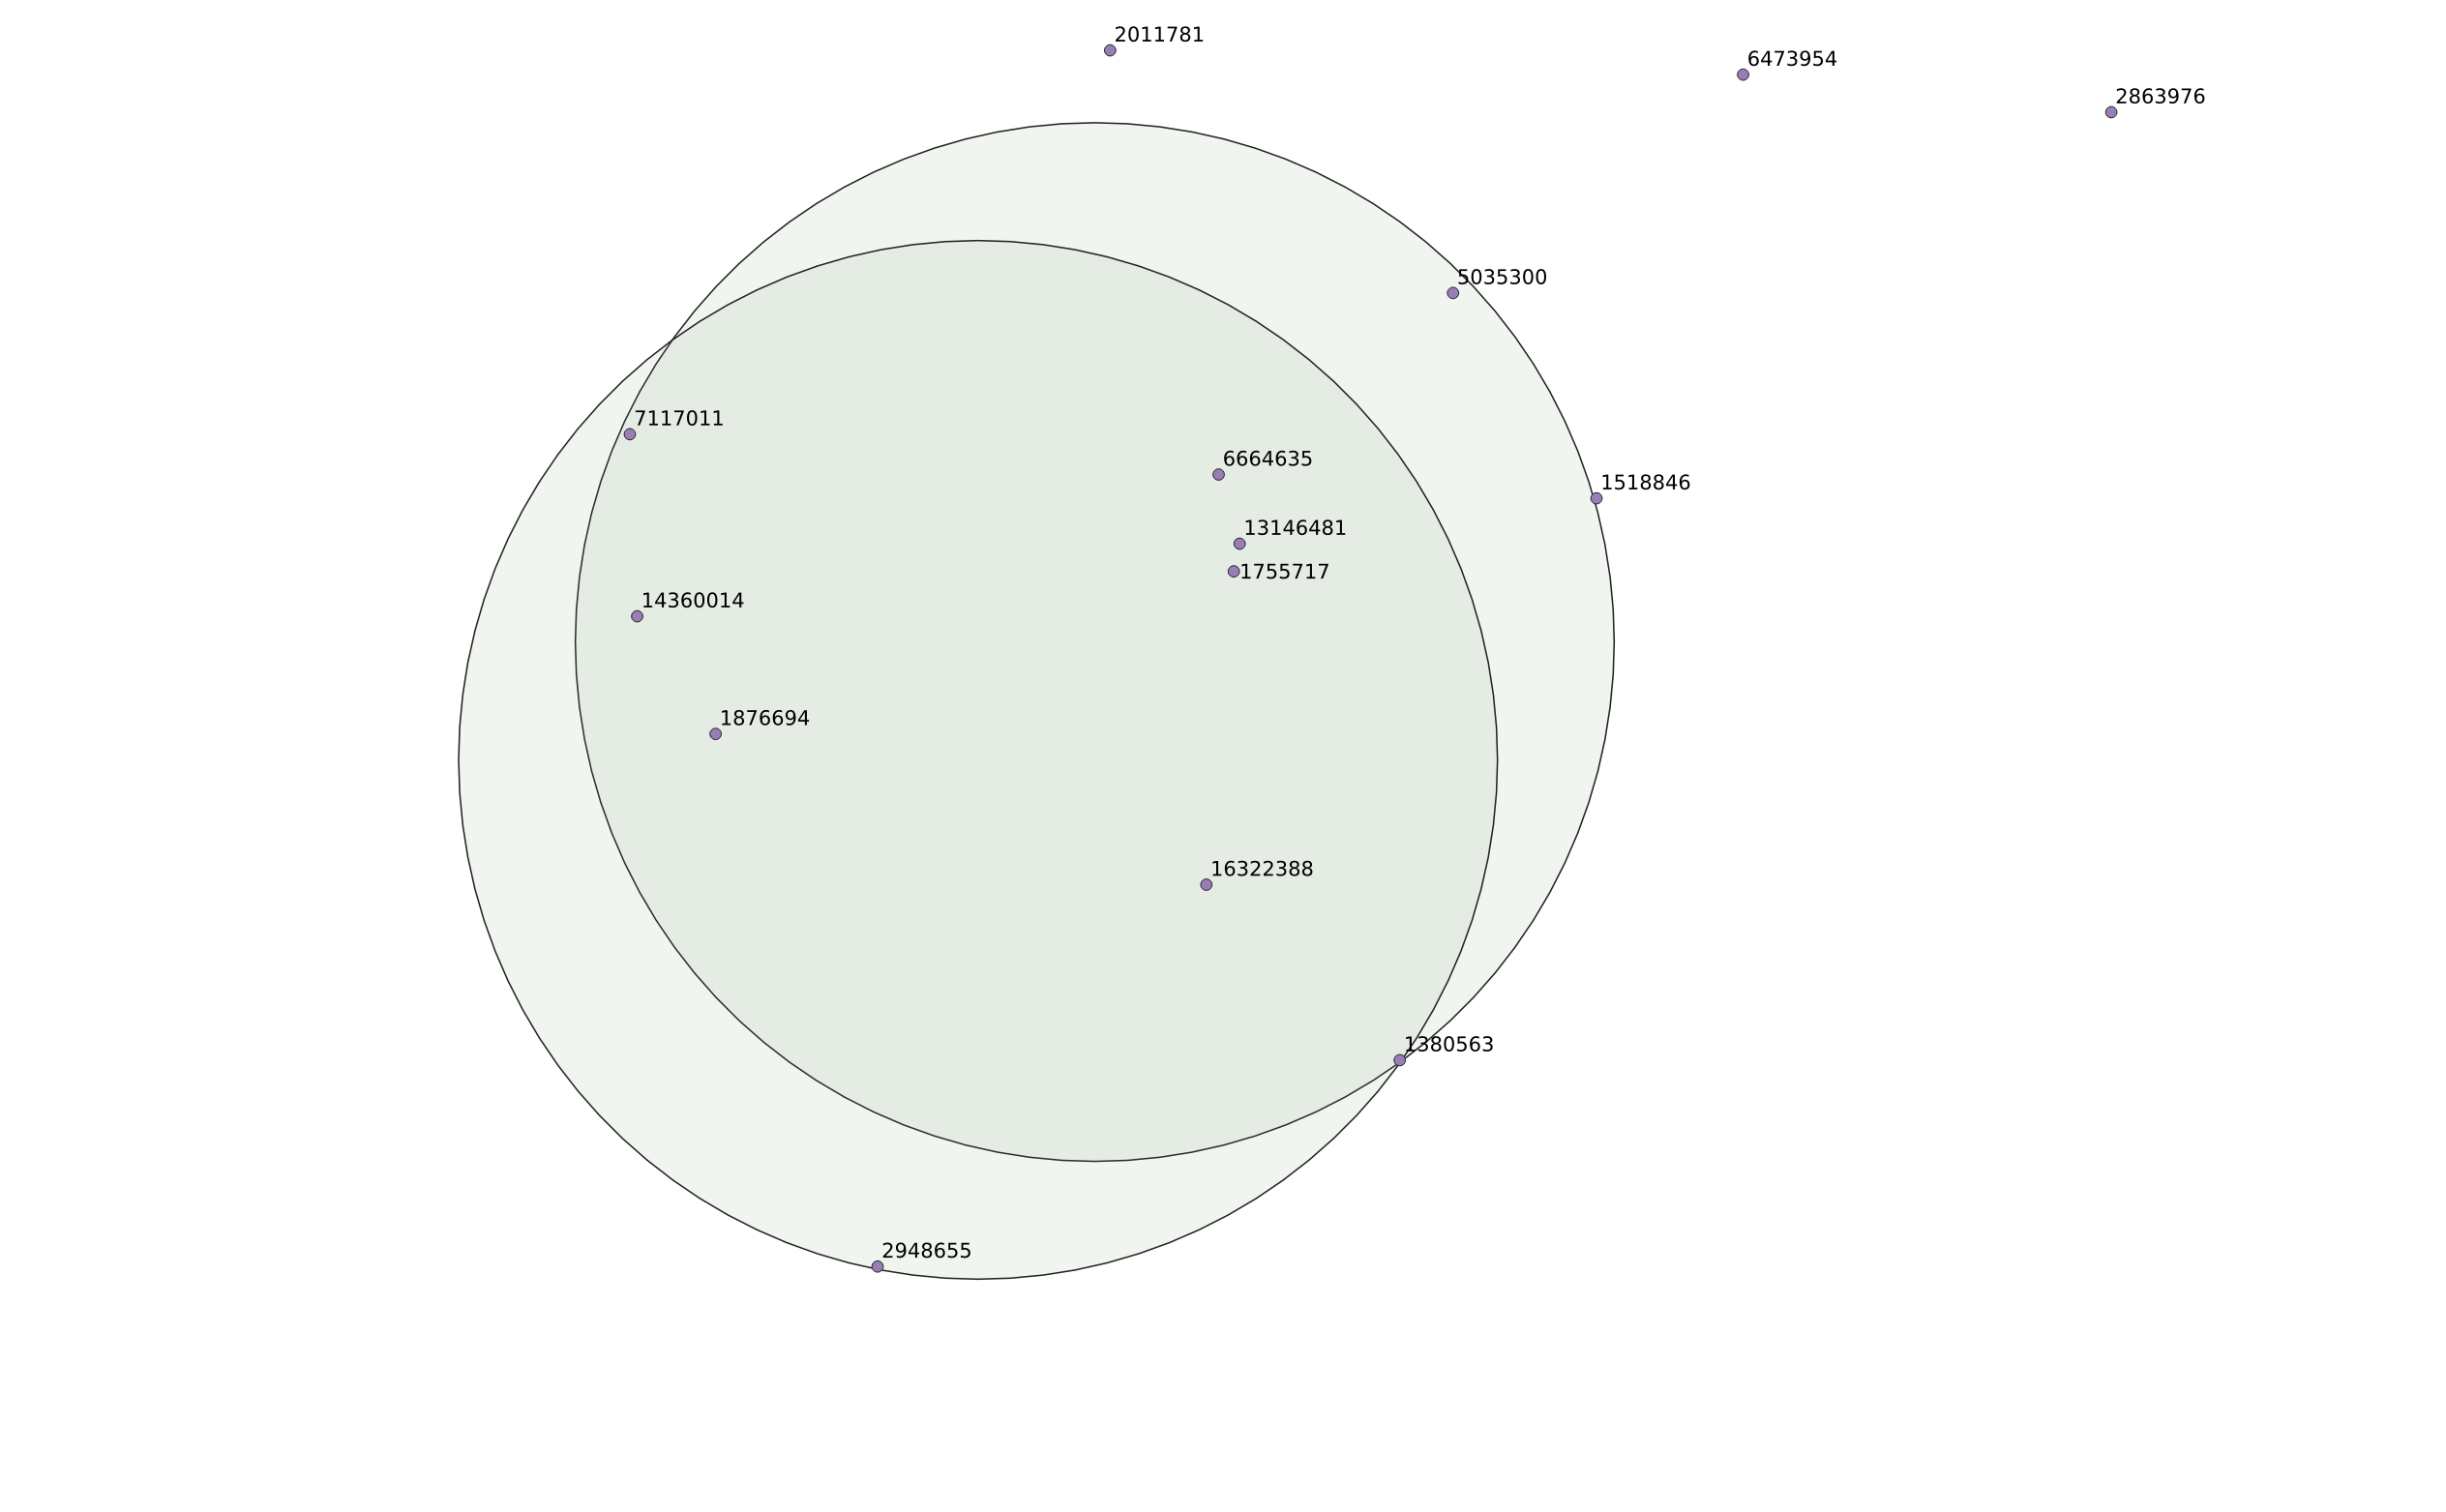
\includegraphics[trim={6cm 2.25cm 6cm 0cm},clip,width=0.7\linewidth]{Figures/t4}
    \scalebox{0.5}{
    \begin{tabular}{c l} \hline
        t& Trajectories in the same disk that \textbf{13805563} \\ \hline
        4&	1518846 1755717 1876694 5035300 6664635 7117011 13146481 14360014 16322388 \\
        4&	1755717 1876694 2948655 6664635 7117011 13146481 14360014 16322388 \\ 
        \hline
    \end{tabular}
    }
\end{frame}

\begin{frame}{Finding maximal patterns using $\delta$ as $min\_sup$ ...}
    
    {\tiny
    \begin{itemize}
     \item The assumption was that maximal patterns will retrieve the largest sets of trajectories which are together. If they happens at least $\delta$ times they should cover the whole window.  However,...
    \end{itemize}
    }
    
    \scalebox{0.45}{
    \begin{tabular}{c l}
        \hline
        t&  Trajectories moving together with \textbf{1380563} \\
        \hline
        0&	1518846 1755717 2011781 2948655 5035300 6664635 13146481 16322388 \\
        0&	1755717 2948655 6664635 7117011 13146481 14360014 16322388 \\
        0&	1755717 2011781 2948655 5035300 6664635 13146481 14360014 16322388 \\
        1&	1518846 1755717 2948655 5035300 6664635 13146481 16322388 \\
        1&	1518846 1755717 2011781 5035300 6664635 13146481 16322388 \\
        1&	1755717 2011781 2948655 5035300 6664635 7117011 13146481 14360014 16322388 \\
        2&	1518846 1755717 1876694 2011781 5035300 6664635 7117011 13146481 14360014 16322388 \\
        2&	1518846 1755717 1876694 2948655 5035300 6664635 13146481 14360014 16322388 \\
        2&	1755717 1876694 2948655 5035300 6664635 7117011 13146481 14360014 16322388 \\
        3&	1518846 1755717 1876694 5035300 6664635 7117011 13146481 14360014 16322388 \\
        3&	1518846 1755717 1876694 2011781 5035300 6664635 13146481 16322388 \\
        3&	1518846 1755717 1876694 2948655 6664635 13146481 16322388 \\
        3&	1755717 1876694 2948655 6664635 7117011 13146481 14360014 16322388 \\
        4&	1518846 1755717 1876694 5035300 6664635 7117011 13146481 14360014 16322388 \\
        4&	1755717 1876694 2948655 6664635 7117011 13146481 14360014 16322388 \\
        \hline
    \end{tabular}
    } \\
    \vspace{0.25cm}
    \scalebox{0.4}{
    \begin{tabular}{l} 
        \hline
        Maximal frequent patterns \\ 
        \hline
        1518846 1755717 1876694 5035300 6664635 13146481 16322388 \\
        1755717 2011781 5035300 6664635 13146481 16322388 \\
        1755717 1876694 2948655 6664635 13146481 16322388 \\
        1755717 2948655 5035300 6664635 13146481 16322388 \\
        1755717 1876694 6664635 7117011 13146481 14360014 16322388 \\
        1755717 2948655 6664635 7117011 13146481 14360014 16322388 \\
        1755717 5035300 6664635 7117011 13146481 14360014 16322388 \\
        1755717 1876694 5035300 6664635 13146481 14360014 16322388 \\
        \hline
    \end{tabular}
    }
\end{frame}

\begin{frame}{Some maximal patterns do not touch all the times...}
    \scalebox{0.45}{
    \begin{tabular}{c l}
        \hline
        t&  Trajectories moving together with \textbf{1380563} \\
        \hline
        0&	1518846 1755717 2011781 2948655 5035300 6664635 13146481 16322388 \\
        0&	1755717 2948655 6664635 7117011 13146481 14360014 16322388 \\
        0&	1755717 2011781 2948655 5035300 6664635 13146481 14360014 16322388 \\
        1&	1518846 1755717 2948655 5035300 6664635 13146481 16322388 \\
        1&	1518846 1755717 2011781 5035300 6664635 13146481 16322388 \\
        1&	1755717 2011781 2948655 5035300 6664635 7117011 13146481 14360014 16322388 \\
        \rowcolor{lightred} 2&	1518846 1755717 1876694 2011781 5035300 6664635 7117011 13146481 14360014 16322388 \\
        \rowcolor{lightred} 2&	1518846 1755717 1876694 2948655 5035300 6664635 13146481 14360014 16322388 \\
        2&	1755717 1876694 2948655 5035300 6664635 7117011 13146481 14360014 16322388 \\
        \rowcolor{lightred} 3&	1518846 1755717 1876694 5035300 6664635 7117011 13146481 14360014 16322388 \\
        \rowcolor{lightred} 3&	1518846 1755717 1876694 2011781 5035300 6664635 13146481 16322388 \\
        3&	1518846 1755717 1876694 2948655 6664635 13146481 16322388 \\
        3&	1755717 1876694 2948655 6664635 7117011 13146481 14360014 16322388 \\
        \rowcolor{lightred} 4&	1518846 1755717 1876694 5035300 6664635 7117011 13146481 14360014 16322388 \\
        4&	1755717 1876694 2948655 6664635 7117011 13146481 14360014 16322388 \\
        \hline
    \end{tabular}
    } \\
    \vspace{0.25cm}
    \scalebox{0.45}{
    \begin{tabular}{l} 
        \hline
        Maximal frequent patterns \\ 
        \hline
        \rowcolor{lightred} 1518846 1755717 1876694 5035300 6664635 13146481 16322388 \\
        1755717 2011781 5035300 6664635 13146481 16322388 \\
        1755717 1876694 2948655 6664635 13146481 16322388 \\
        1755717 2948655 5035300 6664635 13146481 16322388 \\
        1755717 1876694 6664635 7117011 13146481 14360014 16322388 \\
        1755717 2948655 6664635 7117011 13146481 14360014 16322388 \\
        1755717 5035300 6664635 7117011 13146481 14360014 16322388 \\
        1755717 1876694 5035300 6664635 13146481 14360014 16322388 \\
        \hline
    \end{tabular}
    }
\end{frame}

\begin{frame}{More critical, it can hide real patterns...}
    \scalebox{0.45}{
    \begin{tabular}{l} 
        \hline
        Flock hidden by a maximal pattern \\ 
        \hline
        1518846 1755717 5035300 6664635 13146481 16322388 \\
        \hline
    \end{tabular}
    } \\
    \vspace{0.25cm}    
    \scalebox{0.45}{
    \begin{tabular}{c l}
        \hline
        t&  Trajectories moving together with \textbf{1380563} \\
        \hline
        \rowcolor{lightgreen} 0&	1518846 1755717 2011781 2948655 5035300 6664635 13146481 16322388 \\
        0&	1755717 2948655 6664635 7117011 13146481 14360014 16322388 \\
        0&	1755717 2011781 2948655 5035300 6664635 13146481 14360014 16322388 \\
        \rowcolor{lightgreen} 1&	1518846 1755717 2948655 5035300 6664635 13146481 16322388 \\
        1&	1518846 1755717 2011781 5035300 6664635 13146481 16322388 \\
        1&	1755717 2011781 2948655 5035300 6664635 7117011 13146481 14360014 16322388 \\
        \rowcolor{lightgreen} 2&	1518846 1755717 1876694 2011781 5035300 6664635 7117011 13146481 14360014 16322388 \\
        2&	1518846 1755717 1876694 2948655 5035300 6664635 13146481 14360014 16322388 \\
        2&	1755717 1876694 2948655 5035300 6664635 7117011 13146481 14360014 16322388 \\
        \rowcolor{lightgreen} 3&	1518846 1755717 1876694 5035300 6664635 7117011 13146481 14360014 16322388 \\
        3&	1518846 1755717 1876694 2011781 5035300 6664635 13146481 16322388 \\
        3&	1518846 1755717 1876694 2948655 6664635 13146481 16322388 \\
        3&	1755717 1876694 2948655 6664635 7117011 13146481 14360014 16322388 \\
        \rowcolor{lightgreen} 4&	1518846 1755717 1876694 5035300 6664635 7117011 13146481 14360014 16322388 \\
        4&	1755717 1876694 2948655 6664635 7117011 13146481 14360014 16322388 \\
        \hline
    \end{tabular}
    } \\
    \vspace{0.25cm}
    \scalebox{0.45}{
    \begin{tabular}{l} 
        \hline
        Maximal frequent patterns \\ 
        \hline
        \rowcolor{lightred} 1518846 1755717 1876694 5035300 6664635 13146481 16322388 \\
        1755717 2011781 5035300 6664635 13146481 16322388 \\
        1755717 1876694 2948655 6664635 13146481 16322388 \\
        1755717 2948655 5035300 6664635 13146481 16322388 \\
        1755717 1876694 6664635 7117011 13146481 14360014 16322388 \\
        1755717 2948655 6664635 7117011 13146481 14360014 16322388 \\
        1755717 5035300 6664635 7117011 13146481 14360014 16322388 \\
        1755717 1876694 5035300 6664635 13146481 14360014 16322388 \\
        \hline
    \end{tabular}
    }
\end{frame}

\end{document}
